\documentclass[11pt,table]{beamer}
\mode<presentation>
\usepackage{etex}
\usepackage{graphicx}
\usepackage{epstopdf}
\usepackage[english]{babel}
\usepackage{tabularx}
\usepackage{booktabs}
\usepackage{mathrsfs}
\usepackage{multicol}
\usepackage{bm}
\usepackage{subcaption}
\usepackage{wrapfig}
\usepackage{dcolumn}
\usepackage{threeparttable}
\usepackage{booktabs}
\usepackage{bbm}
\usepackage{amsmath,dsfont,listings}
\usepackage{amssymb}
\usepackage{rotating}
\usepackage{multirow}
\usepackage[authoryear]{natbib}
\usepackage{circledsteps}
\usepackage{tikz}
\usetikzlibrary{arrows,decorations.pathmorphing,backgrounds,fit,positioning,shapes.symbols,chains}
\setbeamertemplate{section in toc}[sections numbered]
\setbeamertemplate{caption}[numbered]

\bibliographystyle{Econometrica}

\setbeamersize{text margin right=3.5mm, text margin left=7.5mm}  % text margin
\setbeamersize{sidebar width left=0cm, sidebar width right=0mm}
\setbeamertemplate{sidebar right}{}
\setbeamertemplate{sidebar left}{}

\definecolor{text-grey}{rgb}{0.45, 0.45, 0.45} % grey text on white background
\definecolor{bg-grey}{rgb}{0.66, 0.65, 0.60} % grey background (for white text)
\definecolor{fu-blue}{RGB}{0, 51, 102} % blue text
\definecolor{fu-green}{RGB}{153, 204, 0} % green text
\definecolor{fu-red}{RGB}{204, 0, 0} % red text (used by \alert)

\setbeamertemplate{frametitle}{%
    \vskip-30pt \color{text-grey}\large%
    \begin{minipage}[b][23pt]{80.5mm}%
    \flushleft\insertframetitle%
    \end{minipage}%
}

\setbeamertemplate{navigation symbols}{} 

%%% begin title page
\setbeamertemplate{title page}{
\vskip2pt\hfill
\vskip6pt\hskip3pt

% set the title and the author
\vskip14pt
\parbox[top][1.35cm][c]{11cm}{\LARGE\color{text-grey}\inserttitle \\[1ex] \small \insertsubtitle \\[3ex]}
\vskip11pt
\parbox[top][1.35cm][c]{11cm}{\small \insertauthor \; \insertinstitute \\[2ex] \insertdate}
}
%%% end title page

%%% colors
\usecolortheme{lily}
\setbeamercolor*{normal text}{fg=black,bg=white}
\setbeamercolor*{alerted text}{fg=fu-red}
\setbeamercolor*{example text}{fg=fu-green}
\setbeamercolor*{structure}{fg=fu-blue}

\setbeamercolor*{block title}{fg=white,bg=black!50}
\setbeamercolor*{block title alerted}{fg=white,bg=black!50}
\setbeamercolor*{block title example}{fg=white,bg=black!50}

\setbeamercolor*{block body}{bg=black!10}
\setbeamercolor*{block body alerted}{bg=black!10}
\setbeamercolor*{block body example}{bg=black!10}

\setbeamercolor{bibliography entry author}{fg=fu-blue}
\setbeamercolor{bibliography entry journal}{fg=text-grey}
\setbeamercolor{item}{fg=fu-blue}
\setbeamercolor{navigation symbols}{fg=text-grey,bg=bg-grey}
%%% end colors

%%% headline
\setbeamertemplate{headline}{
\vskip30pt
}
%%% end headline

%%% footline
\newcommand{\footlinetext}{
%\insertshortinstitute, \insertshorttitle, \insertshortdate
}
\setbeamertemplate{footline}{
\vskip2pt
\hfill \raisebox{-1pt}{\usebeamertemplate***{navigation symbols}}
\hfill \insertframenumber\hspace{10pt}
\vskip4pt
}
%%% end footline

%%% settings for listings package
\lstset{extendedchars=true, showstringspaces=false, basicstyle=\footnotesize\sffamily, tabsize=2, breaklines=true, breakindent=10pt, frame=l, columns=fullflexible}
\lstset{language=Java} % this sets the syntax highlighting
\lstset{mathescape=true} % this switches on $...$ substitution in code
% enables UTF-8 in source code:
\lstset{literate={�}{{\"a}}1 {�}{{\"o}}1 {�}{{\"u}}1 {�}{{\"A}}1 {�}{{\"O}}1 {�}{{\"U}}1 {�}{\ss}1}
%%% end listings

\usepackage{concmath}
\usepackage{xcolor}
\definecolor{lightblue}{rgb}{0.8,0.85,1}
\definecolor{persianred}{rgb}{0.8, 0.2, 0.2}
\definecolor{red1}{RGB}{206, 17, 38}
\definecolor{blue1}{RGB}{16, 118, 208}
\definecolor{gray1}{RGB}{117, 115, 115}
\usepackage{hyperref}
\hypersetup{
    bookmarks=false,
    unicode=false,
    pdftoolbar=false,
    pdffitwindow=true,
    pdftitle={Econometricks: Short guides to econometrics},
    pdfauthor={Davud Rostam-Afschar},
    pdfsubject={econometrics},
    pdfcreator={Davud Rostam-Afschar},
    pdfproducer={Davud Rostam-Afschar},
    pdfkeywords={econometrics},
    pdfnewwindow=true,
}

\newtheorem{proposition}{Proposition}
\newtheorem{assumption}{Definition}

\title[] 
{Econome\textcolor{red1}{tricks}: Short guides to econometrics\\[1ex]\normalsize 
}

\author[D. Rostam-Afschar]{Trick 07: Generalized Method of Moments\\[2ex]}

\institute[]{\textcolor{gray1}{Davud Rostam-Afschar (Uni Mannheim)}}
            
\date[] 
{}

\subject{Econometrics}
\renewcommand{\footlinetext}{\insertshortinstitute, \insertshorttitle, \insertshortdate}

\def\sym#1{\ifmmode^{#1}\else\(^{#1}\)\fi}

\begin{document}

\begin{frame}[plain]
  \titlepage
\end{frame}

% --------------------------------------------------- Slide --
\begin{frame}
	\frametitle{Content}
	\tableofcontents[]
\end{frame}
											

\section{How to choose from too many restrictions?}

 %--------------------------------------------------- Slide --
\begin{frame}
	\frametitle{Asymptotic properties of the GMM estimator}
	\tableofcontents[%
 		currentsection, % causes all sections but the current to be shown in a semi-transparent way.
 		currentsubsection, % causes all subsections but the current subsection in the current section to ...
 		%hideallsubsections, % causes all subsections to be hidden.
 		%hideothersubsections, % causes the subsections of sections other than the current one to be hidden.
 		%part=, % part number causes the table of contents of part part number to be shown
 		%pausesections, % causes a \pause command to be issued before each section. This is useful if you
 		%pausesubsections, %  causes a \pause command to be issued before each subsection.
 		%sections={ overlay specification },
	]

\end{frame}


\begin{frame}{Minimize the quadratic form}
\small
The overidentified GMM estimator $\hat{\theta}_{GMM}(W_n)$ for $K$ parameters in $\theta$ identified by $L>K$ moment conditions is a function of the weighting matrix $W_n$ for a sample of $i=1,...,n$ observations:

$$\hat{\theta}_{GMM}(W_n)=\min_\theta q_n(\theta),$$

where the quadratic form $q_n(\theta)$ is the criterion function and is given as a function of the sample moments $\bar{m}_n(\theta)$
$$q_n(\theta)=\bar{m}_n(\theta)'W\bar{m}_n(\theta).$$

The sample moments are a function
$$\bar{m}_n(\theta)=1/n\sum_{i=1}^{N}m(X_i,Z_i,\theta_0)$$
of the model variables $X_i$, the instruments $Z_i$, and the true parameters $\theta_0$.
\end{frame}

\begin{frame}{\small What are the properties of the quadratic form}

$$\underset{\scriptscriptstyle 1\times1}{q_n(\theta)}=\underset{\scriptscriptstyle 1\times L}{\bar{m}_n(\theta)'}\underset{\scriptscriptstyle L\times L}{W}\underset{\scriptscriptstyle L\times1}{\bar{m}_n(\theta)}.$$\\[2ex]

Quadratic form criterion function
$q_n(\theta)\geq0$ is a scalar!\\[2ex]

Weighting matrix $W$ is symmetric (and positive definite that is $x'Wx>0$ for all non-zero $x$)!

\end{frame}



\section{Get the sampling error (at least approximately)}

 %--------------------------------------------------- Slide --
\begin{frame}
	\frametitle{Asymptotic properties of the GMM estimator}
	\tableofcontents[%
 		currentsection, % causes all sections but the current to be shown in a semi-transparent way.
 		currentsubsection, % causes all subsections but the current subsection in the current section to ...
 		%hideallsubsections, % causes all subsections to be hidden.
 		%hideothersubsections, % causes the subsections of sections other than the current one to be hidden.
 		%part=, % part number causes the table of contents of part part number to be shown
 		%pausesections, % causes a \pause command to be issued before each section. This is useful if you
 		%pausesubsections, %  causes a \pause command to be issued before each subsection.
 		%sections={ overlay specification },
	]

\end{frame}


\begin{frame}{\small Get an approximate deviation from the true $\theta_0$}
First order Taylor expansion of sample moments $\bar{m}_n(\hat{\theta}_{GMM})$ around $\bar{m}_n(\theta_0)$ at true parameters gives:

$$\bar{m}_n(\hat{\theta}_{GMM})\approx \bar{m}_n(\theta_0)+\bar{G}_n(\bar{\theta})(\hat{\theta}_{GMM}-\theta_0),$$

where $\bar{G}_n(\bar{\theta})=\frac{\partial \bar{m}_n(\bar{\theta})}{\partial \bar{\theta}'}$ and $\bar{\theta}$ is a point between $\hat{\theta}_{GMM}$ and $\theta_0$.


\end{frame}





\begin{frame}{Check the dimensions}
First order Taylor expansion of sample moments $\bar{m}_n(\hat{\theta}_{GMM})$ around $\bar{m}_n(\theta_0)$ at true parameters gives:

$$\underset{\scriptscriptstyle L\times1}{\bar{m}_n(\hat{\theta}_{GMM})}\approx \underset{\scriptscriptstyle L\times1}{\bar{m}_n(\theta_0)}+\underset{\scriptscriptstyle L\times K}{\bar{G}_n(\bar{\theta})}\underset{\scriptscriptstyle K\times1}{(\hat{\theta}_{GMM}-\theta_0)},$$

where $\bar{G}_n(\bar{\theta})=\frac{\partial \underset{\scriptscriptstyle L\times1}{\bar{m}_n(\bar{\theta})}}{\partial \underset{\scriptscriptstyle 1\times K}{\bar{\theta}'}}$ and $\bar{\theta}$ is a point between $\hat{\theta}_{GMM}$ and $\theta_0$, because of the\\[2ex]
Mean value theorem...

\end{frame}


\begin{frame}{Approximation introduced $\bar{\theta}$}

...where $\bar{G}_n(\bar{\theta})=\frac{\partial \bar{m}_n(\bar{\theta})}{\partial \bar{\theta}'}$ and $\bar{\theta}$ is a point between $\hat{\theta}_{GMM}$ and $\theta_0$.\\[2ex]

Mean value theorem:
$$\bar{G}_n(\bar{\theta})=\frac{\bar{m}_n(\hat{\theta}_{GMM})-\bar{m}_n(\theta_0)}{\hat{\theta}_{GMM}-\theta_0} \text{ for }\theta_0<\bar{\theta}<\hat{\theta}_{GMM}.$$

\begin{figure}
	\centering
		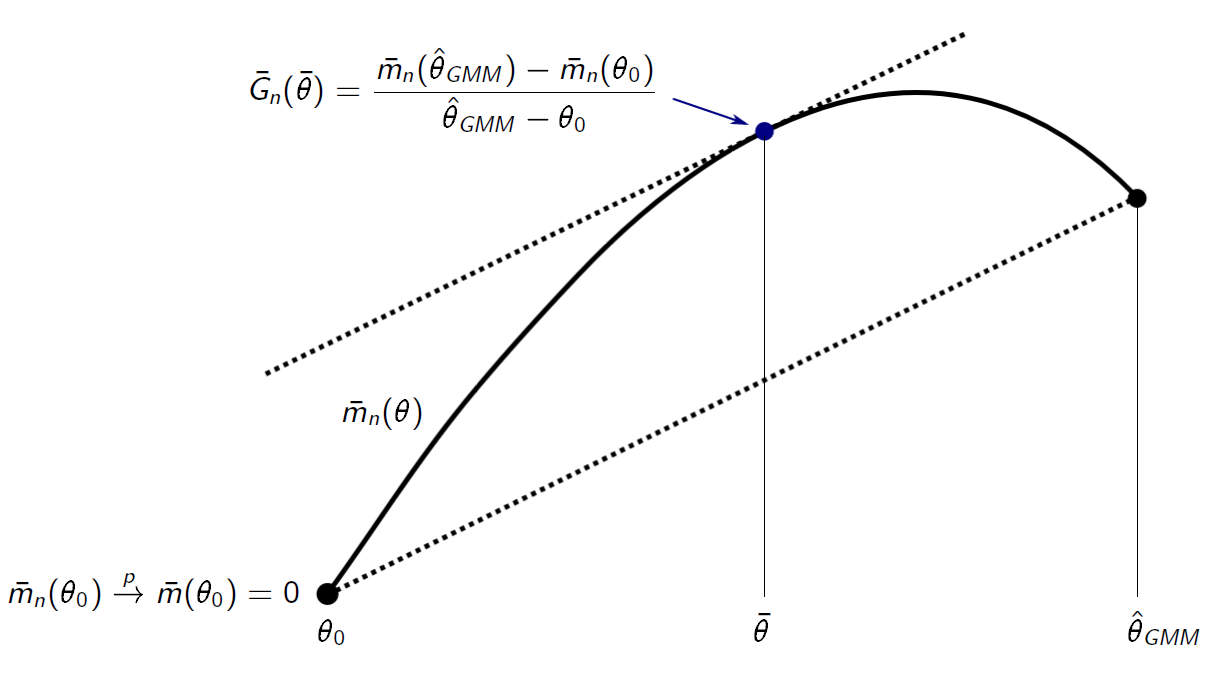
\includegraphics[width=0.50\textwidth]{figures/MeanValueTheorem.png}
	\label{fig:MeanValueTheorem}
\end{figure}


\end{frame}



\begin{frame}{Do the minimization}

To minimize the quadratic form criterion, we take the first derivative of

$$q_n(\theta)=\bar{m}_n(\theta)'W\bar{m}_n(\theta)$$


$$\frac{\partial q_n(\hat{\theta}_{GMM})}{\partial \hat{\theta}_{GMM}}= 2\bar{G}_n(\hat{\theta}_{GMM})'W_n\bar{m}_n(\hat{\theta}_{GMM})=0.$$

\end{frame}


\begin{frame}{Express as much as possible asymptotically}

$$\frac{\partial q_n(\hat{\theta}_{GMM})}{\partial \hat{\theta}_{GMM}}= 2\bar{G}_n(\hat{\theta}_{GMM})'W_n\bar{m}_n(\hat{\theta}_{GMM})=0,$$

Plug in the approximation from before
$$\bar{m}_n(\hat{\theta}_{GMM})\approx \bar{m}_n(\theta_0)+\bar{G}_n(\bar{\theta})(\hat{\theta}_{GMM}-\theta_0)$$

to obtain
$$\bar{G}_n(\hat{\theta}_{GMM})'W_n\bar{m}_n(\theta_0)+\bar{G}_n(\hat{\theta}_{GMM})'W_n\bar{G}_n(\bar{\theta})(\hat{\theta}_{GMM}-\theta_0)\approx0$$



which we rearrange to get the very useful

$$\hat{\theta}_{GMM}\approx \theta_0-(\bar{G}_n(\hat{\theta}_{GMM})'W_n\bar{G}_n(\bar{\theta}))^{-1}\bar{G}_n(\hat{\theta}_{GMM})'W_n\bar{m}_n(\theta_0).$$
So the estimate $\hat{\theta}_{GMM}$ is approximately the true parameter $\theta_0$ plus an sampling error that depends on the sample moment $\bar{m}_n(\theta_0)$.
%$$\sqrt{n}(\hat{\theta}_{GMM}-\theta_0)\approx -(\bar{G}_n(\hat{\theta}_{GMM})'W\bar{G}_n(\bar{\theta}))^{-1}\bar{G}_n(\hat{\theta}_{GMM})'W\sqrt{n}\bar{m}_n(\theta_0),$$

\end{frame}



\begin{frame}{Quickly check dimensions}

Useful approximation
$$\underset{\scriptscriptstyle K\times1}{\hat{\theta}_{GMM}}\approx \underset{\scriptscriptstyle K\times1}{\theta_0}-(\underset{\scriptscriptstyle K\times L}{\bar{G}_n(\hat{\theta}_{GMM})'}\underset{\scriptscriptstyle L\times L}{W_n}\underset{\scriptscriptstyle L\times K}{\bar{G}_n(\bar{\theta})})^{-1}\underset{\scriptscriptstyle K\times L}{\bar{G}_n(\hat{\theta}_{GMM})'}\underset{\scriptscriptstyle L\times L}{W_n}\underset{\scriptscriptstyle L\times1}{\bar{m}_n(\theta_0)}.$$
So the estimate $\hat{\theta}_{GMM}$ is approximately the true parameter $\theta_0$ plus an sampling error that depends on the sample moment $\bar{m}_n(\theta_0)$.


\end{frame}


\section{The econometric model}

 %--------------------------------------------------- Slide --
\begin{frame}
	\frametitle{Asymptotic properties of the GMM estimator}
	\tableofcontents[%
 		currentsection, % causes all sections but the current to be shown in a semi-transparent way.
 		currentsubsection, % causes all subsections but the current subsection in the current section to ...
 		%hideallsubsections, % causes all subsections to be hidden.
 		%hideothersubsections, % causes the subsections of sections other than the current one to be hidden.
 		%part=, % part number causes the table of contents of part part number to be shown
 		%pausesections, % causes a \pause command to be issued before each section. This is useful if you
 		%pausesubsections, %  causes a \pause command to be issued before each subsection.
 		%sections={ overlay specification },
	]

\end{frame}


\begin{frame}{Three assumptions: moment conditions}
\begin{assumption} \textbf{GMM1: Moment Conditions and Identification}. 
$$\bar{m}(\theta_a)\neq\bar{m}(\theta_0)=E[m(X_i,Z_i,\theta_0)]=0.$$
Identification implies that the probability limit of the GMM criterion function is uniquely minimized at the true parameters.
\end{assumption}

\end{frame}

\begin{frame}{Three assumptions: law of large numbers}
\begin{assumption} \textbf{GMM2: Law of Large Numbers Applies}. 
$$\bar{m}_n(\theta)=1/n\sum_{i=1}^{N}m(X_i,Z_i,\theta_0)\overset{p}{\to}E[m(X_i,Z_i,\theta_0)].$$
The data meets the conditions for a law of large numbers to apply, so that we may assume that the empirical moments converge in probability to their expectation.
\end{assumption}
\end{frame}

\begin{frame}{Three assumptions: central limit theorem}
\begin{assumption} \textbf{GMM3: Central Limit Theorem Applies}. 
$$\sqrt{n}\bar{m}_n(\theta)=\sqrt{n}/n\sum_{i=1}^{N}m(X_i,Z_i,\theta_0)\overset{d}{\to}N[0,\Phi].$$
The empirical moments obey a central limit theorem. This assumes that the moments have a finite asymptotic covariance matrix.
\end{assumption}

\end{frame}

\section{Consistency}

 %--------------------------------------------------- Slide --
\begin{frame}
	\frametitle{Asymptotic properties of the GMM estimator}
	\tableofcontents[%
 		currentsection, % causes all sections but the current to be shown in a semi-transparent way.
 		currentsubsection, % causes all subsections but the current subsection in the current section to ...
 		%hideallsubsections, % causes all subsections to be hidden.
 		%hideothersubsections, % causes the subsections of sections other than the current one to be hidden.
 		%part=, % part number causes the table of contents of part part number to be shown
 		%pausesections, % causes a \pause command to be issued before each section. This is useful if you
 		%pausesubsections, %  causes a \pause command to be issued before each subsection.
 		%sections={ overlay specification },
	]

\end{frame}


\begin{frame}{Consistency}
Recall the useful approximation of the estimator:

$$\hat{\theta}_{GMM}\approx \theta_0-(\bar{G}_n(\hat{\theta}_{GMM})'W_n\bar{G}_n(\bar{\theta}))^{-1}\bar{G}_n(\hat{\theta}_{GMM})'W_n\bar{m}_n(\theta_0).$$

Assumption GMM2 implies that $$\bar{m}_n(\theta_0)=1/n\sum_{i=1}^{N}m(X_i,Z_i,\theta_0)\overset{p}{\to}E[m(X_i,Z_i,\theta_0)]=\bar{m}(\theta_0).$$ That is, the sample moment equals the population moment in probability.
Assumption GMM1 implies that $$\bar{m}(\theta_0)=0.$$\\[2ex]

Then $$\bar{m}_n(\theta_0)\overset{p}{\to}\bar{m}(\theta_0)=0,$$
such that $$\hat{\theta}_{GMM}\overset{p}{\to}\theta_0 \text{ for } N\to\infty$$
That is, by GMM1 and GMM2 the GMM estimator is consistent.
\end{frame}



\section{Asymptotic normality}

 %--------------------------------------------------- Slide --
\begin{frame}
	\frametitle{Asymptotic properties of the GMM estimator}
	\tableofcontents[%
 		currentsection, % causes all sections but the current to be shown in a semi-transparent way.
 		currentsubsection, % causes all subsections but the current subsection in the current section to ...
 		%hideallsubsections, % causes all subsections to be hidden.
 		%hideothersubsections, % causes the subsections of sections other than the current one to be hidden.
 		%part=, % part number causes the table of contents of part part number to be shown
 		%pausesections, % causes a \pause command to be issued before each section. This is useful if you
 		%pausesubsections, %  causes a \pause command to be issued before each subsection.
 		%sections={ overlay specification },
	]

\end{frame}


\begin{frame}{Asymptotic normality}
Recall the useful approximation of the estimator:

$$\hat{\theta}_{GMM}\approx \theta_0-(\bar{G}_n(\hat{\theta}_{GMM})'W_n\bar{G}_n(\bar{\theta}))^{-1}\bar{G}_n(\hat{\theta}_{GMM})'W_n\bar{m}_n(\theta_0).$$

Rewrite to obtain
$$\sqrt{n}(\hat{\theta}_{GMM}-\theta_0)\approx -(\bar{G}_n(\hat{\theta}_{GMM})'W_n\bar{G}_n(\bar{\theta}))^{-1}\bar{G}_n(\hat{\theta}_{GMM})'W_n\sqrt{n}\bar{m}_n(\theta_0),$$

The right hand side has several parts for which we made assumptions on what happens when $N\to\infty$. Under the central limit theorem (GMM3)
$$\sqrt{n}\bar{m}_n(\theta_0)\overset{d}{\to}N[0,\Phi]$$

$$plim W_n=W$$
$$plim\bar{G}_n(\hat{\theta}_{GMM})=plim\bar{G}_n(\bar{\theta})=plim\frac{\partial m(X_i,Z_i,\theta_0)}{\partial \theta_0'}=E\bigg[\frac{\partial \bar{m}(\theta_0)}{\partial \theta_0'}\bigg]=\Gamma(\theta_0)$$


\end{frame}


\begin{frame}{Asymptotic normality}
With $plim W_n=W$ and $$plim\bar{G}_n(\hat{\theta}_{GMM})=plim\bar{G}_n(\bar{\theta})=\Gamma(\theta_0)$$

the expression
$$\sqrt{n}(\hat{\theta}_{GMM}-\theta_0)\approx -(\bar{G}_n(\hat{\theta}_{GMM})'W_n\bar{G}_n(\bar{\theta}))^{-1}\bar{G}_n(\hat{\theta}_{GMM})'W_n\sqrt{n}\bar{m}_n(\theta_0)$$

becomes
$$\sqrt{n}(\hat{\theta}_{GMM}-\theta_0)\approx -(\Gamma(\theta_0)'W\Gamma(\theta_0))^{-1}\Gamma(\theta_0)'W\sqrt{n}\bar{m}_n(\theta_0)$$

from which we get the variance $V$. So 
$$\sqrt{n}(\hat{\theta}_{GMM}-\theta_0)\overset{d}{\to}N[0,V]$$
with $$\underset{\scriptscriptstyle K\times K}{V}=1/n[\Gamma(\theta_0)'W\Gamma(\theta_0)]^{-1}[\Gamma(\theta_0)'W\Phi W'\Gamma(\theta_0)][\Gamma(\theta_0)'W\Gamma(\theta_0)]^{-1}$$
That is by GMM1, GMM2, and GMM3 the GMM estimator is asymptotic normal.
\end{frame}

\section{Asymptotic efficiency}

 %--------------------------------------------------- Slide --
\begin{frame}
	\frametitle{Asymptotic properties of the GMM estimator}
	\tableofcontents[%
 		currentsection, % causes all sections but the current to be shown in a semi-transparent way.
 		currentsubsection, % causes all subsections but the current subsection in the current section to ...
 		%hideallsubsections, % causes all subsections to be hidden.
 		%hideothersubsections, % causes the subsections of sections other than the current one to be hidden.
 		%part=, % part number causes the table of contents of part part number to be shown
 		%pausesections, % causes a \pause command to be issued before each section. This is useful if you
 		%pausesubsections, %  causes a \pause command to be issued before each subsection.
 		%sections={ overlay specification },
	]

\end{frame}


\begin{frame}{Asymptotic efficiency}
Which weighting matrix $W$ gives us the smallest possible asymptotic variance of the GMM estimator $\hat{\theta}_{GMM}$.
\small

The variance of the GMM estimator $V$ depends on the choice of $W$
$$V=1/n[\Gamma(\theta_0)'W\Gamma(\theta_0)]^{-1}[\Gamma(\theta_0)'W\Phi W'\Gamma(\theta_0)][\Gamma(\theta_0)'W\Gamma(\theta_0)]^{-1}$$

So let us minimize $V$ to get the \emph{optimal} weight matrix. Try from GMM3
$$\underset{\scriptscriptstyle n\to\infty}{plim} W_n=W=\Phi^{-1}$$

$$V_{GMM,optimal}=1/n[\Gamma(\theta_0)'\Phi^{-1}\Gamma(\theta_0)]^{-1}[\Gamma(\theta_0)'\Phi^{-1}\Phi \Phi^{-1'}\Gamma(\theta_0)][\Gamma(\theta_0)'\Phi^{-1}\Gamma(\theta_0)]^{-1}$$
Which can be simplified to
$$V_{GMM,optimal}=1/n[\Gamma(\theta_0)'\Phi^{-1}\Gamma(\theta_0)]^{-1}$$

\end{frame}


\begin{frame}{Asymptotic efficiency}
$$V_{GMM,optimal}=1/n[\Gamma(\theta_0)'\Phi^{-1}\Gamma(\theta_0)]^{-1}$$
If $\Phi$ is small, there is little variation of this specific sample moment around zero and the moment condition is very informative about $\theta_0$. So it is best to assign a high weight to it.

\begin{figure}
	\centering
		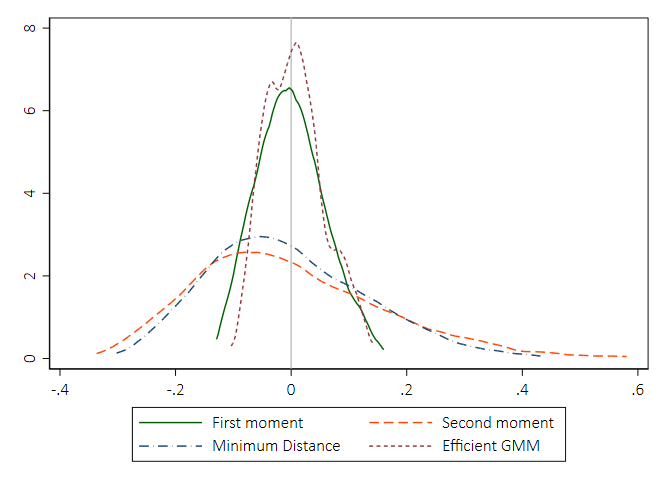
\includegraphics[width=0.50\textwidth]{figures/efficiency.png}
	\label{fig:MeanValueTheorem}
\end{figure}

\end{frame}


\begin{frame}{Asymptotic efficiency}
$$V_{GMM,optimal}=1/n[\Gamma(\theta_0)'\Phi^{-1}\Gamma(\theta_0)]^{-1}$$

 If $\Gamma$ is large, there is a large penalty from violating the moment condition by evaluating at $\theta\neq\theta_0$. Then the moment condition is very informative about $\theta_0$. $V$ is inversely related to $\Gamma$.


\begin{figure}
	\centering
		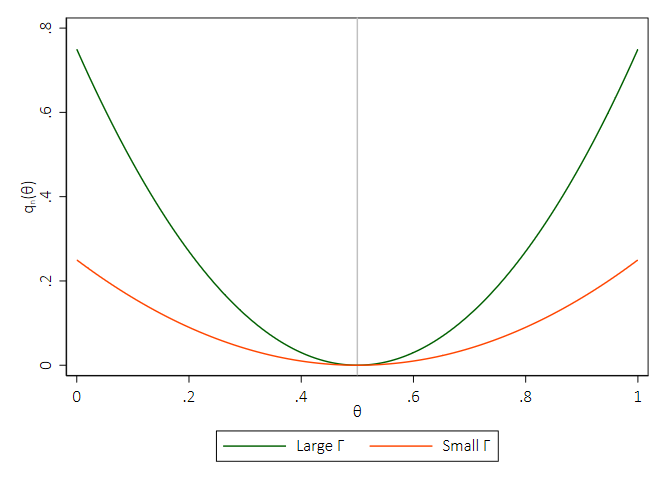
\includegraphics[width=0.50\textwidth]{figures/gamma.png}
	\label{fig:Gamma}
\end{figure}

\end{frame}

\begin{frame}{Estimate the variance in practice}
$$\hat{V}_{GMM,optimal}=1/n[\Gamma(\theta_0)'\Phi_n^{-1}\Gamma(\theta_0)]^{-1}$$

Consistent estimator
$$\Phi_n=NV(\bar{m}_n(\theta))$$

$$\bar{G}_n(\bar{\theta})=\frac{\partial m(X_i,Z_i,\hat{\theta})}{\partial \hat{\theta}'}$$

\end{frame}


\begin{frame}[t,allowframebreaks
]\nocite{*}
\frametitle{References}
\bibliography{bib}
\end{frame}

\end{document}
